\chapter{Automated Planning}
\label{chapter1}
In our daily life, we plan the things we want to do before working them out. The things could be complex tasks like writing a scientific report, they could also be simpler ones like standing up from a seat. When we plan for something, we anticipate the outcomes of actions, then we know what to do (i.e. actions) step by step. Obviously, the planning process is a deliberation process in which we choose and organize actions. The product of the planning is a plan to be performed.

\section{Introduction of Planning}
Automated Planning is the reasoning side of acting. The aim of a planner is to generate a $solution\ plan$ to achieve given $goals$. A planner uses knowledge of the world (e.g. initial world-state, possible actions) to decide what to do before actually performing it.

As in \autoref{fig1_1}, the input world-knowledge of a planning system includes possible $actions$, the $initial\ world$-$state$ of the problem, the objective, etc. the output of the planning system is a $solution\ plan$. The simplest format of a plan is a sequence of actions (i.e. a totally-ordered plan).

\begin{figure}[H]
    \center
    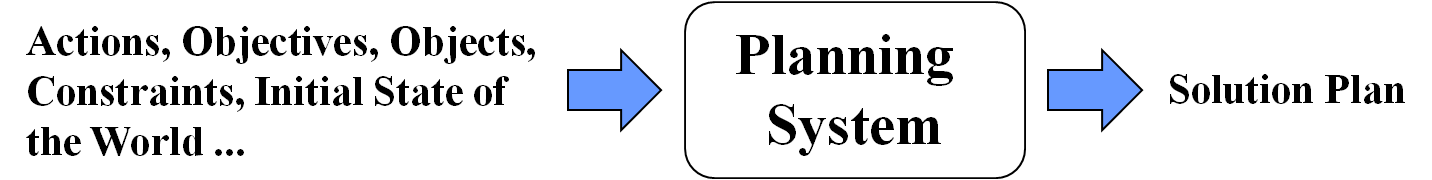
\includegraphics[width=\textwidth]{./images/1_1.png}
    \caption{Planning System}
    \label{fig1_1}
\end{figure}

\begin{itemize}
\item[$\bullet$] \textbf{Initial state}: The state of the world that we start in.
\item[$\bullet$] \textbf{Actions/Operators}: Ways of changing the state of the world.
\item[$\bullet$] \textbf{Objects}: Things in the world that interest us.
\item[$\bullet$] \textbf{Predicates}: Properties of objects, they can be true or false.
\end{itemize}

Different from scheduling in which only certain constraints need to be considered (e.g. time), planning systems must reason about how the world changes to make decisions. Many planners need to keep track of world-state (i.e. the planners need the exact current world state in each step of the planning process). The world state also helps verifying the availability of an action. In planning, each action has a precondition and an effect (or postcondition), the precondition is verified according to the world state, and the effect indicates how the action changes the world state.

Different from reactive system which makes decisions based only on current input, a planning system takes into account the state in the “future” by anticipating the outcomes of actions. 

The action sequences produced by the planning system will be executed by intelligent agents. The system plays an important role to ensure the agents’ rational behavior. The automated planning is widely used in the domains like autonomous robots, space exploration, military logistics, computer games, etc.

\section{Conceptual Model of Planning System}
\label{planningModel}
The conceptual planning system model could be represented as in \autoref{fig1_2}:

\begin{figure}[H]
    \center
    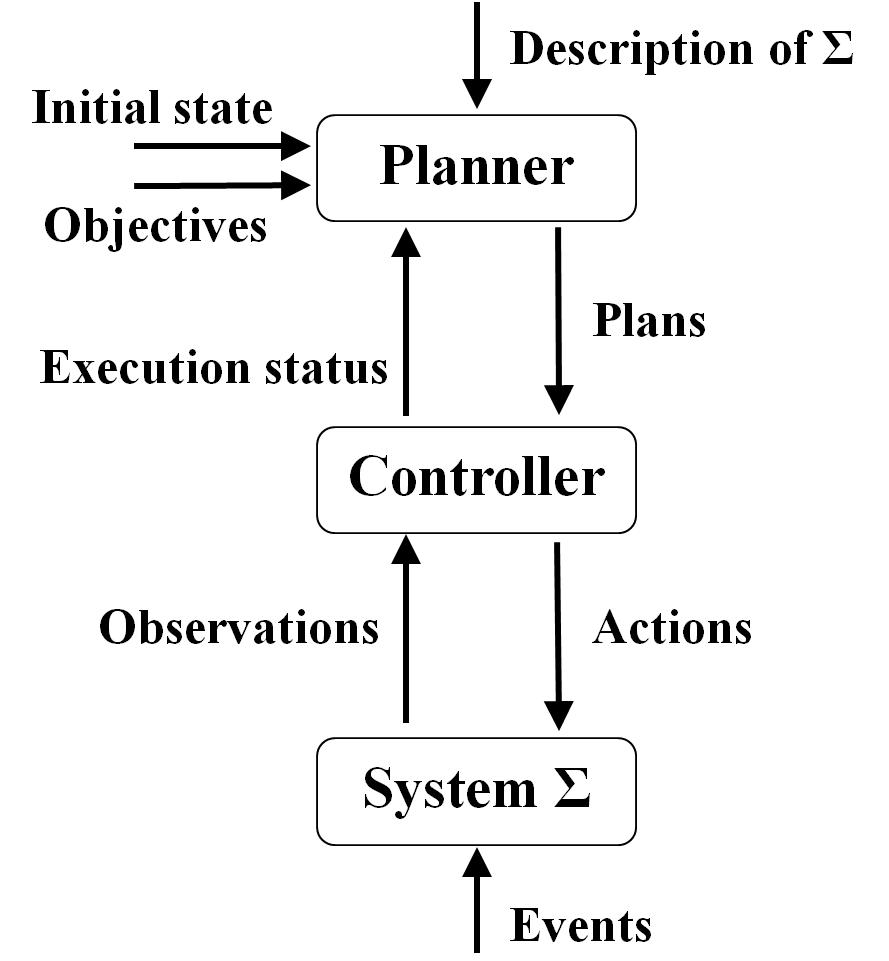
\includegraphics[width=0.5\textwidth]{./images/1_2.png}
    \caption{Conceptual Model}
    \label{fig1_2}
\end{figure}

The model consists of the following three components:
\begin{itemize}\itemsep0pt \parskip1pt \parsep0pt
\item[$\bullet$] A \textbf{planner}, which produces plans and forwards them to the controller as actions to execute;
\item[$\bullet$] A \textbf{controller}, which executes the plan according to observations perceived in the environment;
\item[$\bullet$] A \textbf{state transition system $\Sigma$}, it models the environment in which the plan is to be executed. $\Sigma$ is a 4-tuple, \( $\Sigma = ( S,A,E,\gamma )$\)$\cite{1}$, where
    \begin{itemize}\itemsep0pt \parskip0pt \parsep0pt
    \item[-] $S = \{s_1,s_2,s_3 ...\}$ is a finite or recursively enumerable set of states;
    \item[-] $A = \{a_1,a_2,a_3 ...\}$ is a finite or recursively enumerable set of actions;
    \item[-] $E = \{e_1,e_2,e_3 ...\}$ is a finite or recursively enumerable set of events;
    \item[-] $\gamma$: \(S \times (A \cup E) \rightarrow 2^S \) is a state translation function.
    % \item[]
    \end{itemize}
\end{itemize}

In \autoref{fig1_2}, the execution status is considered only when the planning is online (i.e. the environment is dynamic). Online planning is not discussed in this document. We will consider offline planning only.

\section{Planning Model}
\label{assumptions}
Automated planning is inherently complex and causes large search space. Some planning problems are EXPSPACE-complete. Generally, some assumptions are made to lower the complexity, so that a practical planner can be designed and realized.

The assumptions of a restricted model$ \cite{1}$ and the corresponding assumptions of the extended model$ \cite{1}$ are as follows :

\begin{assumption}[Finite $\Sigma$]
The system $\Sigma$ has a finite set of states in which all the state variables need to be Boolean.
\end{assumption}

\begin{r_assum}
In the system $\Sigma$, there may exist numerical state variables and actions that bring new objects, so infinite set of states must be supported.
\end{r_assum}

\begin{assumption}[Fully observable $\Sigma$]
The system $\Sigma$ is fully observable, i.e. the planner has complete knowledge about the state of $\Sigma$.
\end{assumption}

\begin{r_assum}
The system $\Sigma$ could only be partially observable, i.e. not every aspect of $\Sigma$ can be known.
\end{r_assum}

\begin{assumption}[Deterministic $\Sigma$]
The system $\Sigma$ is deterministic, actions have strictly one possible outcome, i.e. for all s $\in S, u \in A \cup E : \left| \gamma (s,u) \right| \le 1$.
\end{assumption}

\begin{r_assum}
Each action or each event may have multiple alternative effects.
\end{r_assum}

\begin{assumption}[Static $\Sigma$]
The system $\Sigma$ is static, changes in the environement are only caused by actions, there is no external events, i.e. E $= \emptyset$ or $\( \Sigma = ( S,A,\emptyset,\gamma )\)$
\end{assumption}

\begin{r_assum}
There may exist events in the system $\Sigma$. The events change the world state.
\end{r_assum}

\begin{assumption}[Restricted Goals]
The planner holds only restricted goals that are given as an explicit goal state $s_g$ or a set of goal states $S_g$.
\end{assumption}

\begin{r_assum}
More complex objectives may be required, the objective can be not only to reach a given state, but also to satisfy some constraints during the process to the goal state, e.g. some critical states to avoid, some states that must go through.
\end{r_assum}

\begin{assumption}[Sequential Plans]
A solution plan is a linearly finite sequence of actions.
\end{assumption}

\begin{r_assum}
A plan can be partially-ordered. In this case, the plan is no longer a sequence of actions, the orderings between some actions may not be defined.
\end{r_assum}

\begin{assumption}[Implicit Time]
Actions and events have no duration in state translation systems.
\end{assumption}

\begin{r_assum}
Action duration is taken into consideration, so that some temporally constrained goals can be expressed.
\end{r_assum}

\begin{assumption}[Offline Planning]
Planner is not concerned with changes of $\Sigma$ while it is planning.
\end{assumption}

\begin{r_assum}
Planner must consider the dynamic situations of the system, some objectives must be handled online.
\end{r_assum}

The classical planning problem is under the assumptions of the restricted model. Our problem model is under the relaxing assumption 6, and other assumptions of the restricted model.

\section{Domain-Independent Planning}
There are many forms of planning: path and motion planning, perception planning, manipulation planning, communication planning, etc. They are all important domains, there exists some $domain-specific$ planners to solve specific types of problems (path planning, etc). The domain of such a planning system will be specified within the planner, so as in \autoref{fig1_3}, the input of a domain-specific planner only includes the description of a problem.

\begin{figure}[H]
    \center
    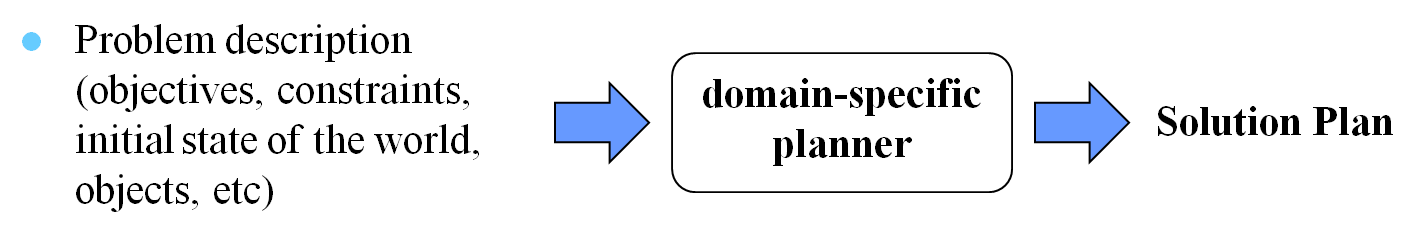
\includegraphics[width=\textwidth]{./images/1_3.png}
    \caption{Domain-specific Planner}
    \label{fig1_3}
\end{figure}

A domain-specific planner works efficiently, but the specification means less flexibility, their algorithms and the data representations are strictly specified. Each of them only solves a certain kind of problem, and when we need to modify the domain, the planner must be modified or even rewritten. On the contrary, a domain-independent planner is a generic planner that solves all kinds of problems. As in \autoref{fig1_4}, the input of a domain-independent planner consists of the descriptions of a problem and a domain.

\begin{figure}[H]
    \center
    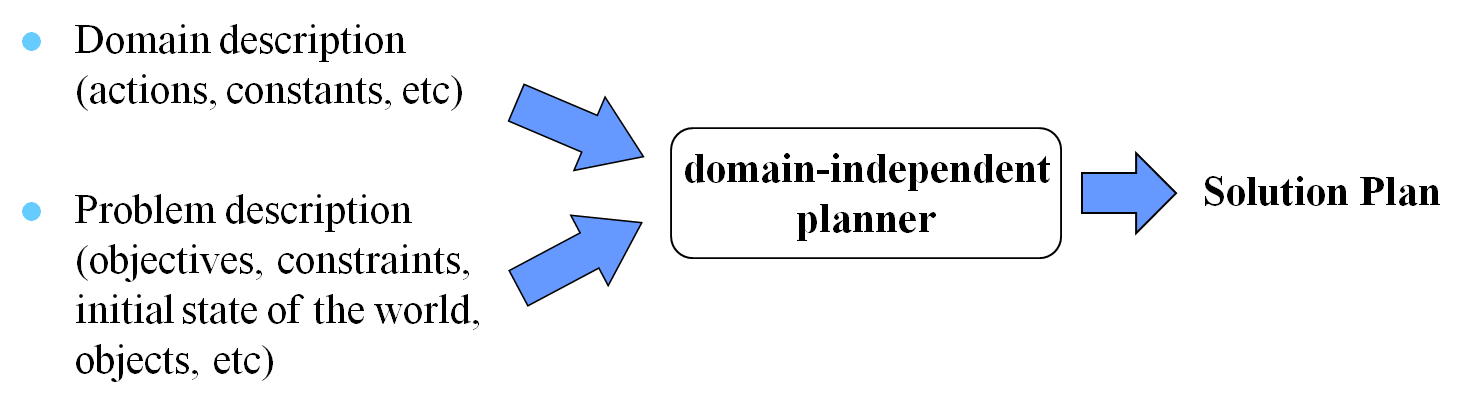
\includegraphics[width=\textwidth]{./images/1_4.png}
    \caption{Domain-Independent Planner}
    \label{fig1_4}
\end{figure}

$Domain-independent$ planners gain flexibility, but their efficiency is more challenging and it requires a general high-level description language to specify the information. For example, Planning Domain Description Language(PDDL) is a standardization of planning domain and problem description languages. In this report, we focus on domain-independent planning.

\section{An example : blocksWorld}
The domain blocksWorld consists of a set of blocks, a table and a set of robot hands. The goal is to arrange the blocks into some given goal stacks. In the domain, we do not care about object positions on the table.

The constraints of blocksWorld are as follows:
\begin{itemize}\itemsep0pt \parskip0pt \parsep0pt
\item[$\bullet$] The blocks can be placed on top of another block or on a table;
\item[$\bullet$] At most one block can be on top of another block, a block that has nothing on it is clear;
\item[$\bullet$] Any number of blocks can be on the table;
\item[$\bullet$] Robot hand can pick up blocks and stack them on other blocks;
\item[$\bullet$] A robot hand can only hold one block or be empty.
\end{itemize}

We have simplified the blocks-world domain which consists of a set of blocks, a single table and a single robot hand, so that some of the constraints (e.g. constraint for multiple hands’ synchronization) are not discussed in this report.

For the simplified blocksWorld domain, the constants of the planning problem are :
\begin{itemize}\itemsep0pt \parskip0pt \parsep0pt
\item A set of blocks \{A, B, C, $\ldots$\}
\end{itemize}

x, y are two blocks, the predicates of the domain are :
\begin{itemize}\itemsep0pt \parskip0pt \parsep0pt
\item[$\triangleright$] \textbf{ontable}(x) : the block x is on the table,
\item[$\triangleright$] \textbf{on}(x,y) : the block x is on top of the block y,
\item[$\triangleright$] \textbf{clear}(x) : there is no block on top of the block x,
\item[$\triangleright$] \textbf{handempty} : the robot hand is empty,
\item[$\triangleright$] \textbf{holding}(x) : the robot hand is holding the block x.
% \item[]
\end{itemize}

A precondition is a set of predicates. An effect is also a set of predicates.

The actions of the domain are : 
\begin{itemize}\itemsep0pt \parskip0pt \parsep0pt
\item[$\triangleright$] \textbf{pickup}(x) : pick up the block x which is currently on the table, x must be clear.
\item[$\triangleright$] \textbf{unstack}(x,y) : pick up the block x which is currently on top of the block y, x must be clear.
\item[$\triangleright$] \textbf{putdown}(x) : put the block x hold by the robot hand on the table.
\item[$\triangleright$] \textbf{stack}(x,y) : put the block x hold by the robot hand on top of the block y, y must be clear.
\end{itemize}

For example, the PDDL definition of the action $pickup$ is as follows:
\\ \hspace*{1.5cm}(:action pickup
\\ \hspace*{2cm}	     :parameters (?x - block)
\\ \hspace*{2cm}	     :precondition (and (clear ?x) (ontable ?x) (handempty))
\\ \hspace*{2cm}	     :effect
\\ \hspace*{2cm}	     (and (not (ontable ?x))
\\ \hspace*{2.5cm}		   (not (clear ?x))
\\ \hspace*{2.5cm}		   (not (handempty))
\\ \hspace*{2.5cm}		   (holding ?x)
\\ \hspace*{2cm})
\\ \hspace*{1.5cm})

In PDDL, a variable begins with the symbol “?”. The parameter of $pickup$ is a block x, its precondition is (clear x) $\wedge$ (ontable x) $\wedge$ (handempty), its effect is (not (ontable x)) $\wedge$ (not (clear x)) $\wedge$ (not (handempty)) $\wedge$ (holding x). The other actions’ PDDL definitions are in \autoref{pddlDomain}.

\begin{figure}[H]
    \center
    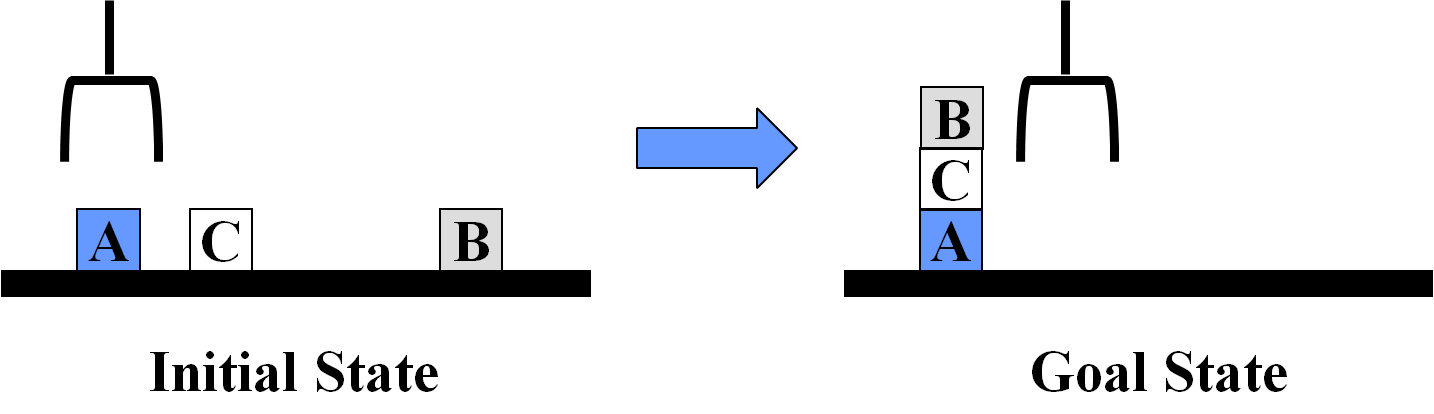
\includegraphics[width=0.8\textwidth]{./images/1_5.png}
    \caption{Planning Problem Example}
    \label{fig1_5}
\end{figure}

\autoref{fig1_5} is an example of the blocks-world planning problem, 
the initial state is : 
clear(a), clear(b), clear(c), ontable(a), ontable(b), ontable(c), handempty
The goal state is : 
on(a,b), on(b,c), ontable(c)

A solution plan is :
pickup(c) $\prec$ stack(c,a) $\prec$ pickup(b) $\prec$ stack(b,c),
the symbol "$\prec$" indicates the ordering of a pair of actions, for example, $A_1$ $\prec$ $A_2$ means that action $A_1$ must finish before $A_2$ starts.

Another solution plan is :
pickup(c) $\prec$ putdown(c) $\prec$ pickup(c) $\prec$ stack(c,a) $\prec$ pickup(b) $\prec$ stack(b,c)

\section{Planning Metrics}
\label{metrics}
The two solutions of \autoref{fig1_5} achieve the same goal. But obviously, the second one has some redundant actions, and the first one is better. The factors that make a solution plan better depends on the application, but some typical plan quality metrics are as follows:
\begin{itemize}\itemsep0pt \parskip0pt \parsep0pt
\item[$\bullet$]\textbf{Plan cost} : every action has a predefined cost, the plan cost is the sum of the cost of actions in the plan;
\item[$\bullet$]\textbf{Plan length} : number of actions in the solution plan;
\item[$\bullet$]\textbf{Makespan} : time to execute the plan.
\end{itemize}

The metrics of a planner are as follows:
\begin{itemize}\itemsep0pt \parskip0pt \parsep0pt
\item[$\bullet$] \textbf{Soundness}: if the planner returns a plan, then this is indeed a solution plan.
\item[$\bullet$] \textbf{Completeness}: if there is a solution plan, then the planner will be able to find the solution plan.
% \item[]
\end{itemize}

If a planner is not complete, it is not guaranteed to find a solution when there exists one. But it is still interesting if an incomplete planner works with high performance. Generally, a planner which is not sound is senseless.

\section{Planning Techniques}
\label{PlanningTechniques}
%Depuis maintenant plus de 30 ans, de nombreuses techniques ont été développées pour répondre au problème de la planification et lever les hypothèses précédemment citées. 
For over 30 years, many techniques have been developed to solve the problem of planning and to remove the assumptions described in \autoref{assumptions}. Among these techniques, $classical planning$ which searches in state-spaces is the simplest. 

Classical planning’s search space can be represented as an oriented graph, in which, each node is a world state, and each arc is an action. State-space planning algorithms searches for a path to the goal state through the graph. Such a path is a solution plan. For example, in \autoref{fig1_6}, each node is a state, each solid arc is an action, the dot arcs indicate that some available actions and their following states are omitted. The node $S_0$ is the initial state, $S_1$ is the goal state. In the graph, there exists a path from $S_0$ to $S_1$ which is “stuck(C,B) $\prec$ unstuck(C,A)”, this path is a solution plan.

\begin{figure}[H]
    \center
    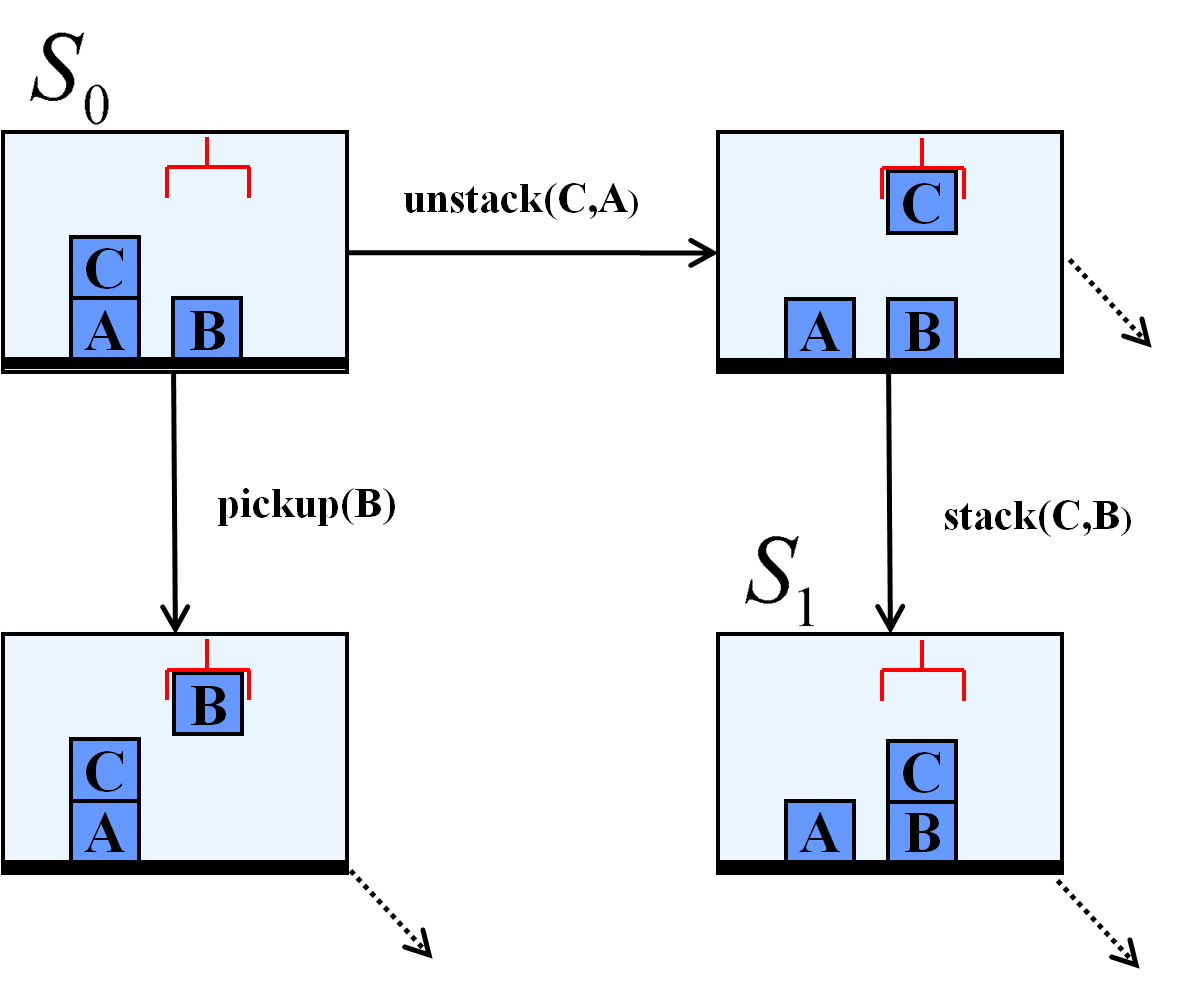
\includegraphics[width=0.65\textwidth]{./images/1_6.png}
    \caption{State Search Space}
    \label{fig1_6}
\end{figure}

The planning algorithm generates part of the whole search space to find a path to goal state (i.e. to find a solution plan). In classical planning, there are several kinds of algorithms, such as forward search which is from the initial state towards the goal state. With the knowledge of the current state (at the beginning of the search, the current state is the initial state), forward search only tries available actions from the current node. Then the following states are obtained according to the effects of the action on the current state. The algorithm repeats this procedure until it reaches a goal state or the search has covered the whole graph.

%Récemment, les planificateurs reposant sur cette technique couplée à une recherche en chaînage avant et à une heuristique qui estime la distance au but en ignorant les effets négatifs des actions, ont permis à la planification d’effectuer un saut quantitatif en termes de performance [RW08, HN01]. 

%Les techniques de recherche dans un espace de plans [PW92] fonctionnent par ranements successifs d’un plan, jusqu’à ce que tous les conflits entre les actions et toutes les préconditions des actions soient produites par une autre action du plan ou bien étant vérifiées dans l’état initial. 

There are many planning techniques which are different from classical planning. For example, some techniques search in $plan-spaces$ \cite{PW92}, they work by successively repairing a plan until all conflicts are removed.

%Les techniques utilisant des graphes de planification [BF97] reposent sur deux idées : une analyse d’atteignabilité et une technique de ranement disjonctive, qui consiste à adresser un ou plusieurs conflits en utilisant une disjonction de résolveurs. 

The planning techniques using $graphs$ \cite{BF97} are based on two ideas: reachability analysis and disjunctive repairing technique, which solves one or more conflicts by using a disjunction of resolvers. 

%Les techniques Sat (SATisfiability problem) encodent le problème de planification sous la forme d’un problème de satisfiabilité et effectuent ensuite la recherche d’un plan solution en s’appuyant sur des algorithmes Sat connus [RG08, KS98a]. 
%Le problème de planification peut être également encodé sous la forme d’un problème Csp (Constraints Satisfaction Problem) [Kam00, PV08]. Pour les deux dernières techniques, l’idée sous-jacente est de bénéficier directement des avancées dans ces deux domaines. 

The $SAT$ techniques (SATisfiability problem) encode a planning problem as a satisfiability problem and then search for a solution based on known SAT algorithms \cite{RG08}\cite{KS98a}. A planning problem can also be encoded as a CSP (Constraints Satisfaction Problem) problem \cite{Kam00}\cite{PV08}. The idea of these two techniques is to benefit directly from the advantages in the two areas.

%Les techniques Htn (Hierarchical Transition Network) sont similaires aux techniques de recherche dans les espaces d’états dans la mesure ou` chaque état est représenté par un ensemble de propositions. Toutefois, les planificateurs Htn [NAI+03, EHN94] diffèrent dans leur façon de chercher un plan puisqu’ils fonctionnent par décomposition récursive d’une tâche complexe en tâches primitives. 

%Avec les techniques Mdp (Markov Decision Process) [MT08, SWD08], le problème de planification consiste à développer une politique optimale, i.e., à associer à un état une action qui maximise une récompense globale. Cette dernière technique est largement adoptée pour traiter les problèmes de planification non-déterministe. 

With $MDP$ (Markov Decision Process) techniques \cite{MT08}, \cite{SWD08}, the planning problem is converted to develop an optimal policy, i.e. to associate a state with an action that maximizes the global reward. This technique is widely used to treat non-deterministic planning problems. 

%Finalement, des techniques issues du Model Checking [PT01] permettent de planifier en prenant en compte l’incertitude, le non-déterminisme et l’observabilité partielle de l’environnement.

The techniques developed from $Model Checking$ \cite{PT01} take uncertainty, nondeterminism and partial observability of the environment into account.

Finally, $HTN$ (Hierarchical Transition Network) planners \cite{3}\cite{4} differ in the way to search for a plan, they decompose compound tasks recursively to primitive tasks. More details will be discussed in \autoref{chapter2}.

%Planning is a search process, which searches in a certain search space.